% TODO:
% Use 'IoT'
% Mention outreach? - perhaps to introduce the graph section
% Ensure that what is written here about Bluetooth working with our setup if a set of devices is provided is correct
% Sort out tenses
% Pictures of the equipment

We implemented a test bed for future development of a security protocol. Our proof-of-concept used standard IoT components to produce our architecture and move data over it, demonstrating common features of a larger IoT system.

% ✔ We wanted to make a prototype for use as a test bed (or proof-of-concept) for future development of an IoT security protocol, blah.
% ✔ Chose to use off-the-shelf component for maximum applicability, blah


\subsection{Equipment}
\paragraph{}
For Edge Devices, we used Arduino Unos which are inexpensive (£25-30), low powered and portable making them a popular choice for IoT. With 14 inputs and outputs (analog and digital), these microcontrollers can be loaded with pre-compiled programs to read from sensors and write to outputs. To communicate with Smart Agents, we used Serial over either USB or Bluetooth (through the addition of a HC-05 Bluetooth module - see Figure \ref{fig:HC-05}).


\begin{figure}
    \centering
    \includegraphics[width=0.5\textwidth]{HC05.jpg}
    \caption{The HC-05 chip for serial over Bluetooth. It costs roughly £4 and has a range of about 10m. Requiring a pin to pair the devices, it can have the role of either slave (wait for connection passively) or master (search for the device and actively initiate connection).}
    \label{fig:HC-05}
\end{figure}

\paragraph{}
As Smart Agents, we used the Raspberry PI 3 which is a single board computer. Communication with Edge Devices and the Cloud was possible without any additional adapters over USB, Ethernet, WiFi and Bluetooth. The PI can run PC scale applications headless on its Linux operating system. Its low price, small form factor and low power requirement make it popular for IoT.

\paragraph{}
We used STFC's SCD Cloud for access to a virtual machine running Scientific Linux 7. A common LAN enabled TCP/IP communication between this machine and the Smart Agents or the web application.

% ✔ We used Arduino Unos (£25-30) as edge devices. They have X inputs and outputs (analog and digital) and can be loaded with pre-compiled programs.
% ✔ HC-05 chip for Bluetooth option (picture of HC-05, range=10m?, cost=£4...)
% ✔ Raspberry pi as smart agents. Stats – 1GB RAM, can be run headless, use linux...
% ✔ SCD Cloud machine (Scientific Linux 7) hugely useful, blah.

\subsection{Setup}

\begin{figure}
    \centering
    \includegraphics[width=0.5\textwidth]{Architecture.png}
    \caption{The architecture we implemented.}
    \label{fig:architecture}
\end{figure}

\paragraph{}
The Cloud VM was setup as the MQTT broker using Mosquitto. There were three endpoints contacting it: Smart Agents, Broker Services and the web application. Using the Paho MQTT client library for Python as well as the PyBluez module, the Smart Agents acted as a gateway to the Cloud for any connected Edge Devices. If one Smart Agent could not directly connect to the hub, Bluetooth tethering was used to share the connection of a nearby Smart Agent. Broker Services ran on the Cloud as a Python application (also using Paho) to publish a list of currently connected devices for discovery. A Flask module (Flask-MQTT) served a web application, allowing a user to subscribe to topics for an overview of the data flows in the network.

\paragraph{}
There were several problems with using Bluetooth. In our initial setup, the HC-05s were configured in slave mode with names according to a pattern. The Smart Agent would periodically scan for new devices according to the pattern and then attempt to connect. However, with only one Bluetooth chip, each PI could not send/receive while scanning so communications experienced a substantial delay (roughly 20s). To counter this, we used a fixed list of Edge Devices per Smart Agent which were always available. While seemingly restrictive, this would work adequately for a variety of use cases - such as a central Smart Agent controlling statically placed sensors in a house or vehicle. Additionally, the number of devices in each piconet was restricted to seven. This didn't affect our prototype but may be an issue for scaling in a real setup.

\paragraph{}
Depending on the use case, different communication technologies may be more applicable. With Edge Devices that are relatively fixed, our serial protocol worked over USB - where there was no delay to scanning but was it was not wireless. Some protocols that are wireless - such as Zigbee - can connect a larger number of devices but require bespoke hardware at both ends. Our technique of sending a JSON encoded packet could work on any text communication protocol - we implemented it over USB and Bluetooth serial.

\paragraph{}
Edge devices interacted directly with each sensor, sending JSON packets of tagged data for the Smart Agent to forward to the broker. The programs were written in C and were compiled and uploaded using the Arduino IDE.


\begin{figure}
    \centering
    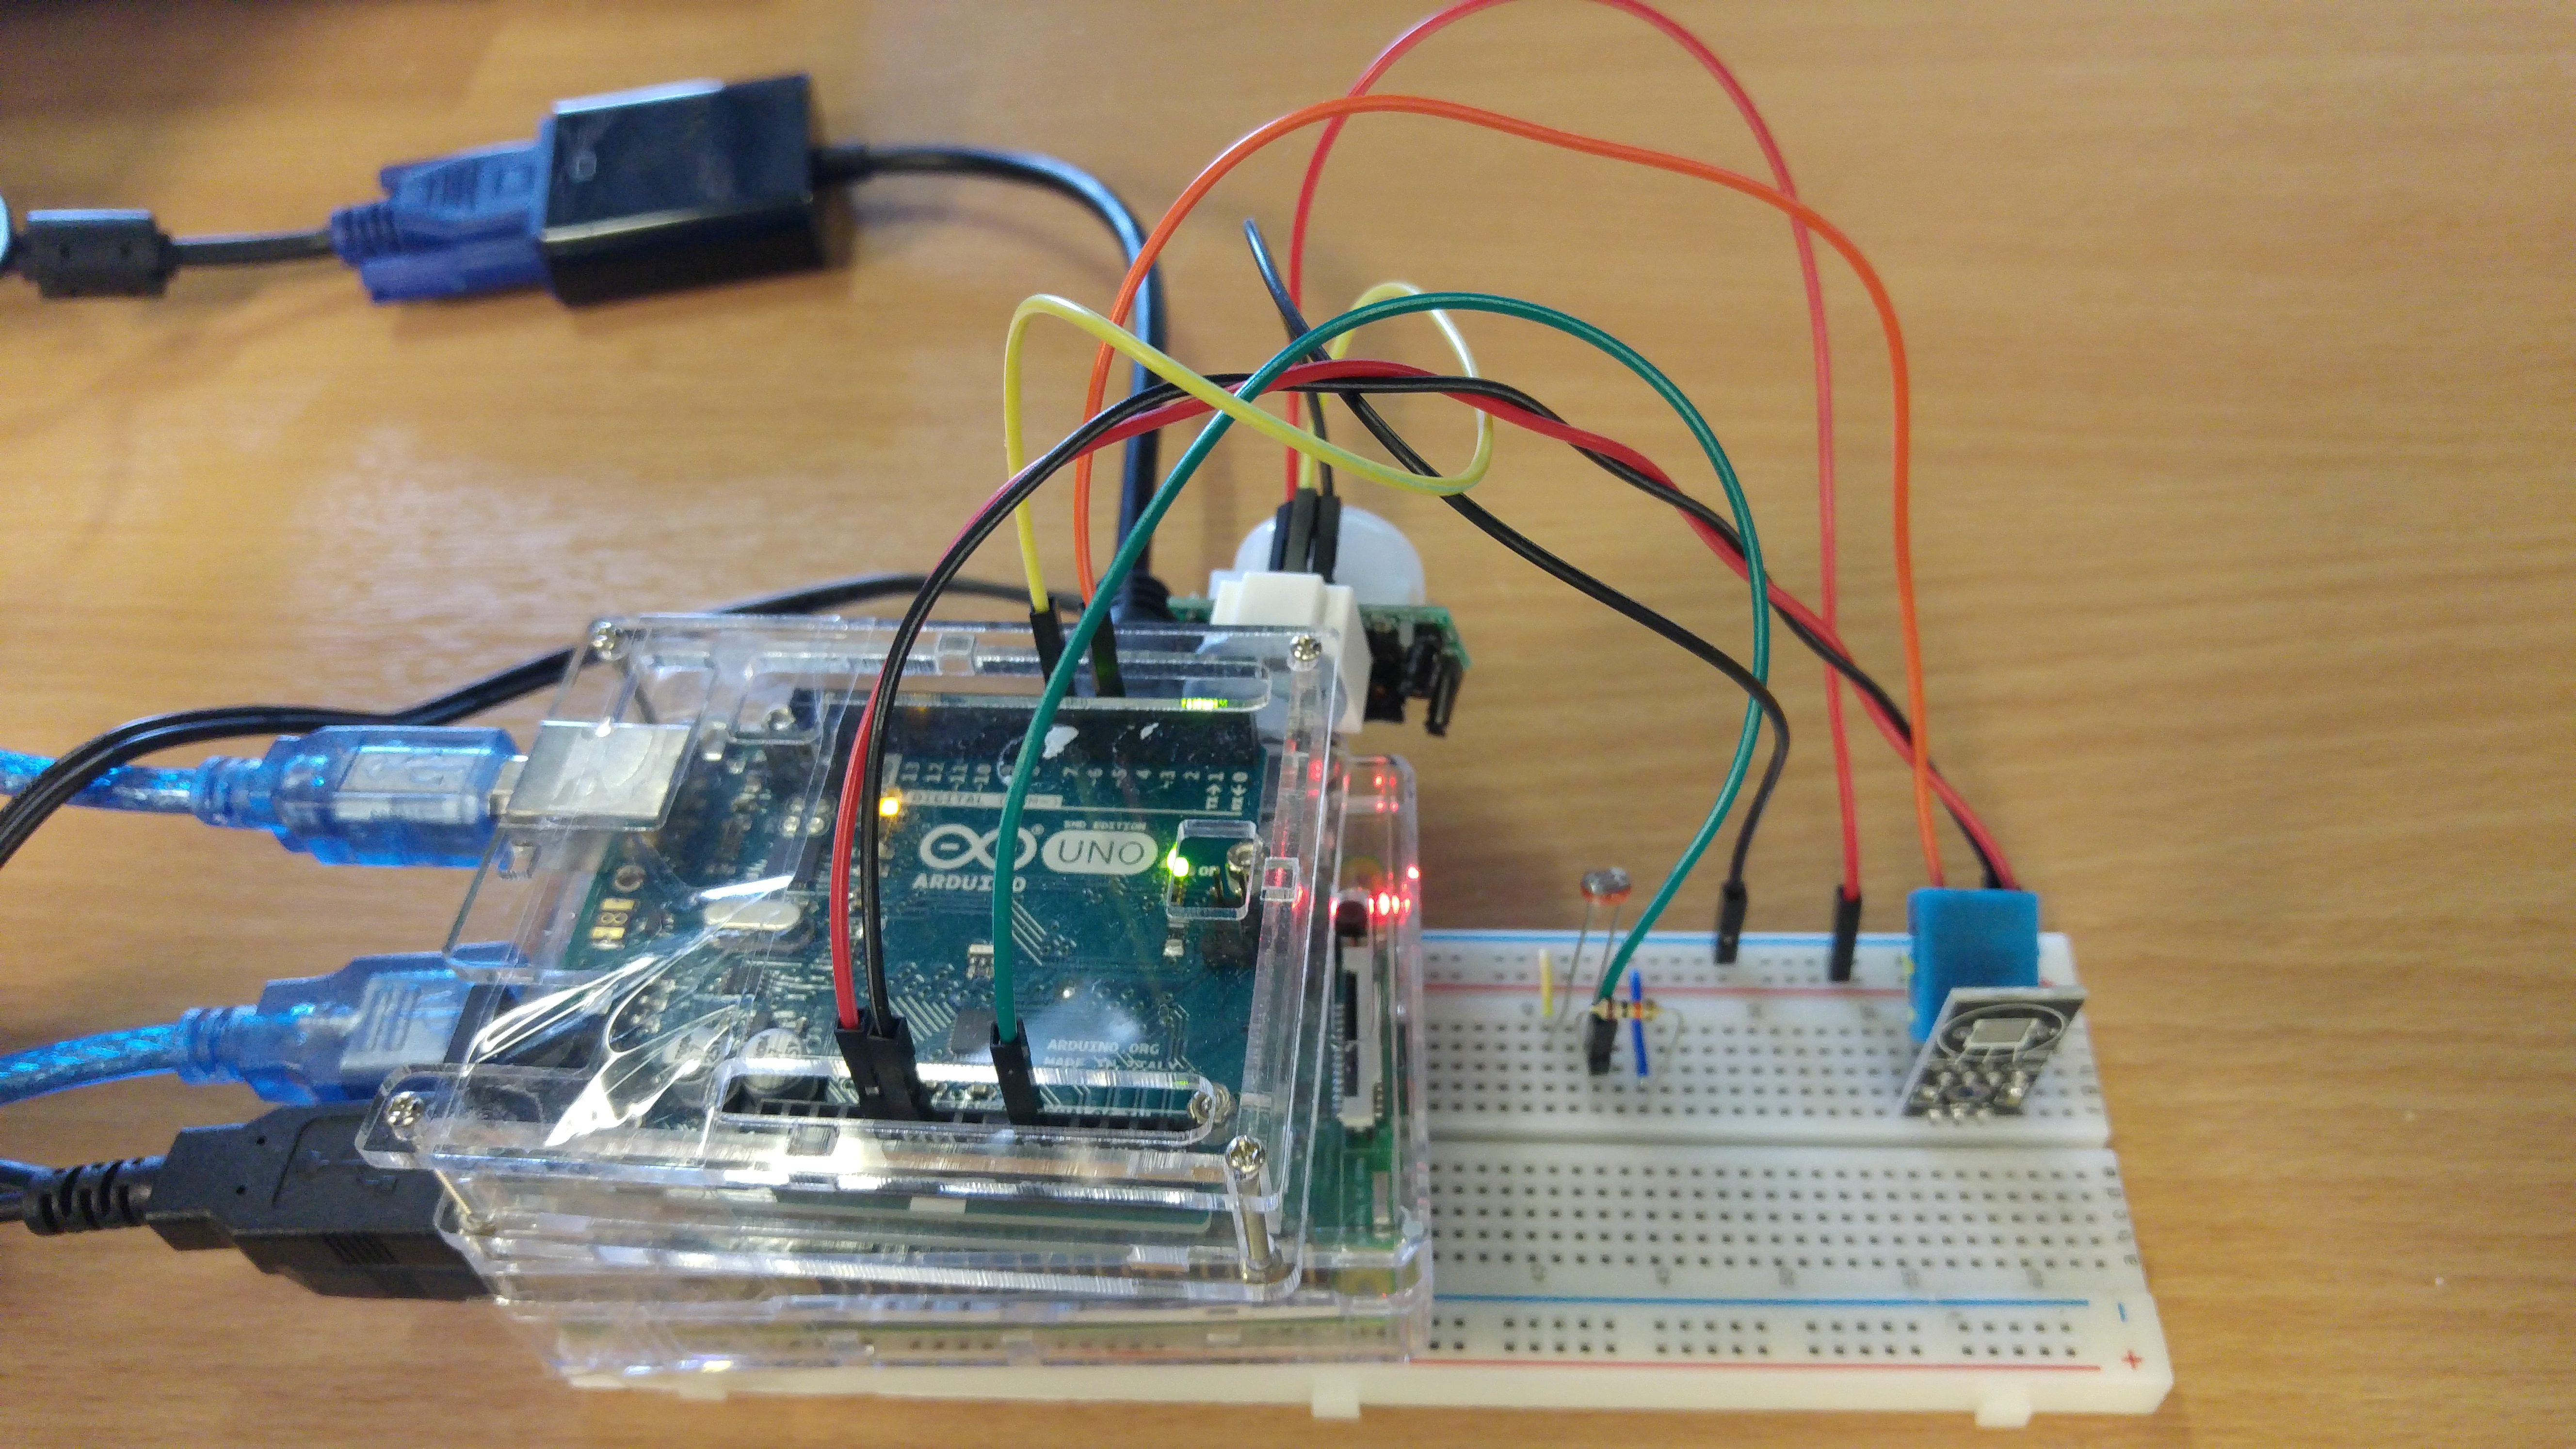
\includegraphics[width=0.7\textwidth]{setup.jpg}
    \caption{A Raspberry PI (bottom) connected to an Arduino (top) relaying data to the MQTT broker in the Cloud passed from the Arduino which is reading the attached sensors.}
    \label{fig:setup}
\end{figure}

% ✔ Each edge device is identified by a unique ID which is a random number
% ✔ Communication between Smart Agent and Edge via Bluetooth.
% What is Bluetooth /why is it a good option for communicating with low memory/power/connectivity devices? PAIRING!
% ✔ Smart agents run Piduino to interface between MQTT Pub/Sub and the inputs and outputs in the edge
% ✔ Broker (mosquitto) runs on cloud, as does telemetry and monitoring applications (broker services) and a flask app.
% Pretty diagrams and pictures of the equipment
% ✔ Diagram with the pretty logos on it I made for the pre-coffee talk. I’ll go find it.
% ✔ Line about PI talks to PI


\subsection{Data}

\begin{figure}
    \centering
    \begin{tikzpicture}
    \begin{axis}[
        title={Light Intensity over the 28th and 29th June},
        xlabel={Time [HH:MM]},
        ylabel={Arduino Reading [5V / 1024]},
        xlabel near ticks,
        date coordinates in=x,
        xticklabel style={rotate=90,
                          anchor=near xticklabel},
        xticklabel=\hour:\minute,
        ymajorgrids=true,
        xmajorgrids=true,
        grid style=dashed,
        legend pos=outer north east,
        legend entries={Emma,Callum},
    ]
        \addplot [blue, mark=none] table [x=Datetime,y=Emma, col sep=tab] {LDR_dates.tsv};
        \addplot [orange, mark=none] table [x=Datetime,y=Callum, col sep=tab] {LDR_dates.tsv};
    \end{axis}
    \end{tikzpicture}
    \caption{The data collected by different Arduinos, aggregated in the Cloud after being published to the MQTT broker via the Smart Agents. The light intensity is recorded as the voltage over an LDR.}
    \label{fig:graph}
\end{figure}

\paragraph{}
Figure \ref{fig:graph} shows an example of data that was collected during a test of our system. Using four Smart Agents at different places around the office overnight, we connected Edge Devices with sensors whose data was published to the MQTT broker for recording. Including LDRs, Thermistors and Humidity sensors, the different combination of detectors attached to each device demonstrated the system handling various data streams concurrently.

\paragraph{}
The data itself is interesting. Emma's sensor - which was closer to a window - shows a steeper increase in light intensity in the morning compared to Callum's where the most significant increase comes later, from the lights turning on. At different points during the night (particularly around 9:15 at Callum's desk) the lights were turned back on indicating that someone returned to the office or something triggered their movement sensors. We used this setup as a part of STFC outreach events to record similar data for visiting children to analyse.

% ✔ Also used for outreach activities, blah
% ✔ Pretty graph of some data collected
% ✔ Graph, and also some brief waffle about what’s on the graph.
